\documentclass[a4paper]{article}

\usepackage{a4wide}
\usepackage[utf8]{inputenc}
\usepackage[ngerman]{babel}
\usepackage{fancyhdr}
\usepackage{graphicx}
\usepackage[parfill]{parskip}
\usepackage{color}

% fuer "deko-elemente"
\pagestyle{fancy}

% we needs moar platz
\topmargin -5mm
\headheight 20mm

% include logo in document head
\chead{
\includegraphics[width=50mm]{logo.pdf}}

% seitenzahl entfernen
\cfoot{}

% footer content
\lfoot{\small{AlphaLabs}}
\rfoot{\tiny{Alexander Drangmeister, Dennis Esders, Philipp Heisig, Robert Baruck, Stephan Wilde, Kilian Költzsch}}

% headrule
\renewcommand\headrule{
\vspace{3mm}
\footrule
}

% footrule
\renewcommand\footnoterule{\rule{\linewidth}{0pt}}

% change standard font
\usepackage[T1]{fontenc}
\newcommand{\changefont}[3]{
\fontfamily{#1} \fontseries{#2} \fontshape{#3} \selectfont}

% Tagesordnungspunkt Item
\newcommand{\TOP}[1]{\item \textbf{#1}\par}



\begin{document}
\changefont{cmss}{m}{n} %computer modern sans serif

\begin{center}
\textbf{\Large The Circle of Waste - Teilziel 4}
\end{center}

\vspace{5mm}

% ich weiss leider wirklich nicht was LaTeX hier fuer ein bescheuertes Problem hat, aber ich entschuldige mich aufrichtig fuer diesen "Format-Spam", irgendwann™ schaue ich mir das mal genauer an, so ist das ja ne zumutung m(
\definecolor{dgreen}{rgb}{0.549,0.776,0.247}
\makeatletter
\def\footrule{{
  \vskip-\footruleskip\vskip-\footrulewidth
  \color{\footrulecolor}
  \hrule\@width\headwidth\@height
  \footrulewidth\vskip\footruleskip
}}
\makeatother
\renewcommand{\footrulewidth}{3pt}
\newcommand{\footrulecolor}{dgreen}

\begin{enumerate}

%%%%%%%%%%%%%%%%%
% HIER GEHT'S LOS
%%%%%%%%%%%%%%%%%

\TOP{Strukturübersicht}

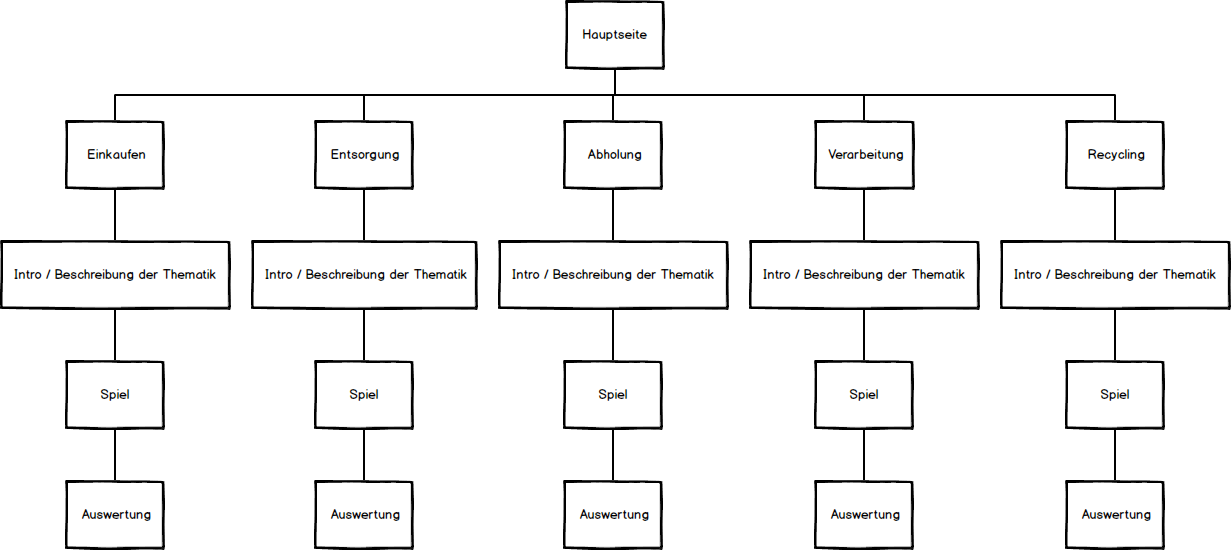
\includegraphics[width=\linewidth]{struktur.png}

Wir haben ein Hauptmenü von dem alle freigeschalteten Unterkapitel erreicht werden können. Diese werden in linearer Reihenfolge freigeschaltet, können aber mehrfach durchlaufen werden und enden jeweils wieder im Hauptmenü.

\TOP{Kapitel 1}
\textbf{Inhalt}\\
Das erste Kapitel behandelt einige Beispiele, bei denen im Alltag Müll erzeugt wird wie z.B. beim Kochen oder bei bestimmten Hobbies. Außerdem werden Charaktere vorgestellt, die im späteren Verlauf des Spiels zum Teil wieder vorkommen.\\
\textbf{Erwartungsbild}\\
Der Benutzer entwickelt ein Verständnis für den im Alltag entstehenden Müll und wie dieser verringert werden kann.\\
\textbf{Reaktion auf Fehler}\\
Fehler bei der Einschätzung von produziertem Müll werden als solche erfasst und es wird erläutert, wieso es sinnvollere Einschätzungen gibt. Zusätzlich werden Tipps zum praktischen Umgang mit diesem Müll gegeben.\\
\textbf{Einodnung in Lerntheorie}\\
Unser 1. Kapitel verknüpft verschiedene Lerntheorien, im Speziellen folgende Punkte:\\
\begin{enumerate}

\item Behaviorismus
  \begin{enumerate}
    \item Lernen als Suchprozess mit Verstärkung der zufällig richtigen Reaktion\\
    Phase 1 - Falls der Benutzer die Antwort nicht weiß hat er noch die Möglichkeit eine zufällige Antwort auszuwählen, diese wird ihm dann ggf. durch einen Applaus als richtige Antwort dargestellt.
  \end{enumerate}
  
\item Kognitivismus
  \begin{enumerate}
    \item Lernen als vielschichtiger Prozess der Informationsverarbeitung zur Erzeugung innerer Strukturen\\
    Es wird in Phase 1 (Gedächtnisspiel) versucht den Benutzer dazu zu bewegen verschiedene alltägliche Tätigkeiten ins Gedächtnis zu rufen und Stück für Stück mit Charakteren aus dem Spiel zu verknüpfen. Im Folgenden wird in Phase 2 von dem Benutzer verlangt diese bereits bekannten Tätigkeiten mit ihrem Müllausstoß und Ideen zur Vermeidung in Verbindung zu bringen.
    \item Wissen nicht als eingepaukte Information, sondern durch Verstehen und Verarbeiten von Informationen erwerben\\
    Im Phase 2 wird von dem Nutzer erwartet sich mit verschiedenen Tätigkeiten auseinanderzusetzen und diese hinsichtlich ihres Müllausstoßes zu bewerten, im Folgenden wird dem Benutzer durch weitere Informationen die Chance gegeben, seine eigenen Ideen mit gegebenen zu vergleichen.
  \end{enumerate}
  
\item Konstruktivismus
  \begin{enumerate}
    \item Lernen als kein passives Aufnehmen und Abspeichern von Informationen sondern aktiver Prozess der Wissenskonstruktion\\
    In Phase 1 wird von dem Benutzer verlangt bereits bekannte Begriffe eigenständig mit seinem Wissensnetzwerk zu verknüpfen um sich möglichst gut daran zu erinnern. In Phase 2 muss der Benutzer diese dann aufgrund ihres Müllausstoßes selbst einordnen und bewerten.
  \end{enumerate}

\end{enumerate}
            
Zusammenfassend geht es in unserem ersten Kapitel darum, den Nutzer langsam an das Thema Müll heranzuführen, indem zuerst gezielt bereits bekanntes Wissen abgerufen und neu verknüpft wird und im Folgenden dieses Wissen in einen Bezug zu Müll gebracht und entsprechend bewertet wird. Hierbei wird der Spieler durch Zeitliche begrenzung motiviert und aufmerksam gehalten, sowie durch ein Punktesystem angespornt.


\TOP{Kapitel 2}
\textbf{Grundidee}\\
Das Spiel ist zu einem kleinen Teil bereits implementiert.\\
Im Grunde besteht das Spiel aus zwei Phasen. In Phase 1 muss der Spieler verschiedene zufällig ausgewählte Müllsorten, ähnlich wie bei Tetris, in eine passende Mülltonne fallen lassen.\\
Daraufhin wird in Phase 2 Analysiert wo bei dem Zuordnen Fehler aufgetreten sind und es wird auf Fehlverhalten hingewiesen.Außerdem werden weiterführende Informationen zum besseren Verständnis geliefert.\\
\textbf{Inhalt}\\
Im 2. Kapitel wird die richtige Trennung von Müll behandelt, wozu verschiedene Müllobjekte wie zB. Apfelreste, Bananen oder Glasflaschen, als auch Müllbehälter wie blaue Tonnen, schwarze Tonnen oder Glascontainer miteinander verknüpft werden.\\
\textbf{Erwartungsbild}\\
Der Spieler lernt auf unterhaltsame und fordernde Weise, wo er verschiedensten Müll richtig entsorgt.\\
\textbf{Reaktion auf Fehler}\\
Auftretende Fehler in Phase 1 werden gespeichert und es wird in Phase 2 explizit auf diese eingegangen um Fehlverhalten zu identifizieren und zu verbessern.\\
\textbf{Einodnung in Lerntheorie}\\
Unser 2. Kapitel verknüpft verschiedene Lerntheorien, vor allem folgende Punkte:\\
\begin{enumerate}


\item Behaviorismus
  \begin{enumerate}
    \item Lernen als Konditionierungsvorgang\\
    In Phase 1 wird durch das Richtige Zuordnen verschiedener Müllsorten in die passenden Behälter je nach Richtigkeit positive oder negative Reize in Form von Punkten gesetzt.
    \item Lernen als Suchprozess mit Verstärkung der zufällig richtigen Reaktion\\
     Falls nicht bereits im Vorfeld bekannt lernt der Spieler in Phase 1 durch Ausprobieren, ob ein Müllobjekt in einen bestimmten Behälter gehört.
  \end{enumerate}
  
\item Kognitivismus
  \begin{enumerate}
    \item Lernen als vielschichtiger Prozess der Informationsverarbeitung zur Erzeugung innerer Strukturen\\
   Es werden dem Spieler in Phase 1 durch Wiederholung die Grundlagen \glqq eingehämmert\grqq\ um eine Wissensbasis zu schaffen, woraufhin in Phase 2 Informationen die zu Fehlern führten und weitere Informationen besser mit der bereits geschaffenden Basis verknüpft werden können.
  \end{enumerate}
  
\item Konstruktivismus
  \begin{enumerate}
    \item Lernen nur durch aktive Beteiligung des Lernenden\\
    Der Benutzer agiert direkt mit verschiedenen Müllobjekten und Müllbehältern, indem er diese manuell verschieben und austauschen muss, wodurch er den direkten Umgang mit diesen stärker verinnerlicht.
  \end{enumerate}

\end{enumerate}
            
Zusammenfassend  geht es in unserem zweiten Kapitel darum, den Nutzer in der 1. Phase durch Wiederholung der selbst zuzuordnenden Gegenstände und direkter Resonanz, die richtige Trennung von Müll zu \glqq erkunden\grqq zu lassen. Im Folgenden werden in Phase 2 Quellen die zu Fehlverhalten geführt haben behandelt und Missverständnisse aus dem Weg geräumt.

%%%%%%%%%%%%%%%%%%%
% HIER IST'S VORBEI
%%%%%%%%%%%%%%%%%%%

\end{enumerate}


% das ist herrlich kompliziert, aber es klappt! das ist alles was zaehlt! :D
\definecolor{dgreen}{rgb}{0.549,0.776,0.247}
\makeatletter
\def\footrule{{
  \vskip-\footruleskip\vskip-\footrulewidth
  \color{\footrulecolor}
  \hrule\@width\headwidth\@height
  \footrulewidth\vskip\footruleskip
}}
\makeatother
\renewcommand{\footrulewidth}{3pt}
\newcommand{\footrulecolor}{dgreen}

\end{document}
